\chapter{Results}
\label{ch:results}

\section{Stage 1 Results Overview}
\label{sec:results-overview}

Stage 1 constitutes the principal empirical contribution of this thesis: a systematic evaluation of the AMATAS v2 two-tier architecture across all fourteen attack types present in the CICIDS2018 NetFlow v3 dataset. Each experiment comprised 1,000 flows sampled at a realistic class distribution --- 50 attack flows and 950 benign flows (a 5\% attack prevalence), ordered chronologically by source IP and flow start time to preserve the temporal structure that the AMATAS temporal agent relies upon. All experiments employed GPT-4o as the underlying language model for the six-agent pipeline, with the Tier 1 Random Forest pre-filter operating at a classification threshold of 0.15 --- a setting established during development to achieve 100\% recall on the training partition whilst incurring zero false positives (Appendix B).

Table~\ref{tab:stage1-results} presents the full per-experiment results across all 14,000 flows.

\begin{table}[H]
\centering
\caption{Stage 1 Per-Experiment Results ($n = 1{,}000$ flows per experiment; 50 attack + 950 benign)}
\label{tab:stage1-results}
\small
\begin{tabularx}{\textwidth}{l r r r r r r r r r}
\toprule
Attack Type & TP & FP & FN & TN & Recall & FPR & F1 & Cost (\$) & Filter Rate \\
\midrule
FTP-BruteForce & 50 & 0 & 0 & 950 & 100.0\% & 0.00\% & 100.0\% & 2.13 & 95.0\% \\
SSH-Bruteforce & 49 & 0 & 1 & 950 & 98.0\% & 0.00\% & 99.0\% & 2.16 & 94.9\% \\
DoS-SlowHTTPTest & 50 & 0 & 0 & 950 & 100.0\% & 0.00\% & 100.0\% & 2.12 & 95.0\% \\
DoS-Slowloris & 50 & 0 & 0 & 950 & 100.0\% & 0.00\% & 100.0\% & 2.16 & 95.0\% \\
DoS-Hulk & 46 & 0 & 4 & 950 & 92.0\% & 0.00\% & 96.0\% & 2.17 & 95.0\% \\
DoS-GoldenEye & 46 & 0 & 4 & 950 & 92.0\% & 0.00\% & 96.0\% & 2.15 & 95.0\% \\
DDoS-LOIC-HTTP & 41 & 0 & 9 & 950 & 82.0\% & 0.00\% & 90.0\% & 1.57 & 95.0\% \\
DDoS-LOIC-UDP & 50 & 4 & 0 & 946 & 100.0\% & 0.42\% & 96.2\% & 1.87 & 94.1\% \\
DDoS-HOIC & 29 & 1 & 21 & 949 & 58.0\% & 0.11\% & 73.4\% & 1.79 & 94.1\% \\
Bot & 41 & 6 & 9 & 944 & 82.0\% & 0.63\% & 85.4\% & 2.30 & 92.7\% \\
Infiltration & 0 & 2 & 50 & 948 & 0.0\% & 0.21\% & 0.0\% & 0.80 & 97.4\% \\
Brute\_Force-Web & 43 & 4 & 7 & 946 & 86.0\% & 0.42\% & 89.1\% & 2.05 & 93.3\% \\
Brute\_Force-XSS & 42 & 2 & 8 & 948 & 84.0\% & 0.21\% & 89.3\% & 2.09 & 93.7\% \\
SQL\_Injection & 49 & 3 & 1 & 947 & 98.0\% & 0.32\% & 96.1\% & 1.99 & 94.0\% \\
\midrule
\textbf{Aggregate} & \textbf{586} & \textbf{22} & \textbf{114} & \textbf{13,278} & \textbf{83.7\%} & \textbf{0.07\%} & \textbf{86.3\%} & \textbf{27.35} & \textbf{94.4\%} \\
\bottomrule
\end{tabularx}

\vspace{0.5em}
\noindent\textit{FPR = False Positive Rate (FP / (FP + TN)); F1 = harmonic mean of precision and recall; Filter Rate = proportion of flows classified as benign by Tier 1 without LLM invocation.}
\end{table}

\begin{figure}[H]
\centering
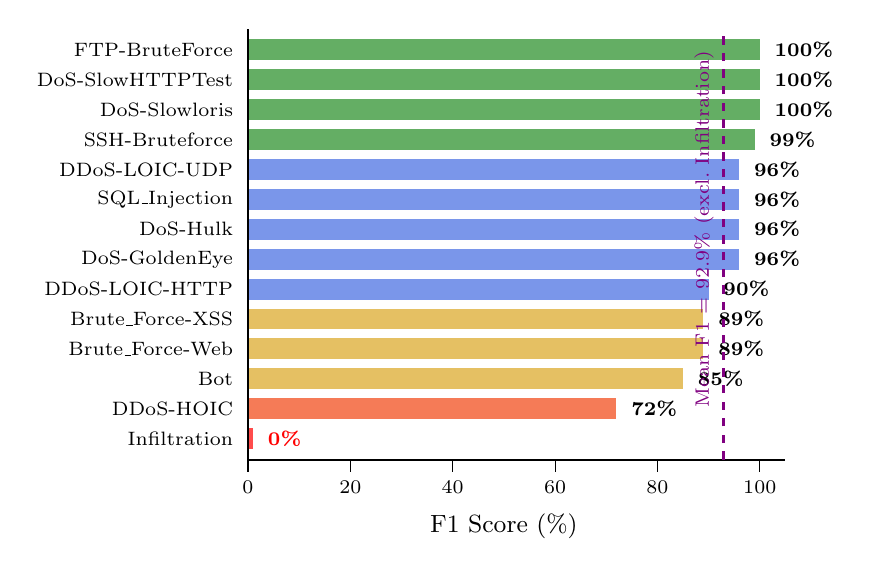
\begin{tikzpicture}[y=0.38cm, x=0.065cm]

% Draw bars individually (sorted by F1 descending)
\foreach \name/\val/\col/\ypos in {
  FTP-BruteForce/100/ForestGreen/13,
  DoS-SlowHTTPTest/100/ForestGreen/12,
  DoS-Slowloris/100/ForestGreen/11,
  SSH-Bruteforce/99/ForestGreen/10,
  DDoS-LOIC-UDP/96/RoyalBlue/9,
  SQL\_Injection/96/RoyalBlue/8,
  DoS-Hulk/96/RoyalBlue/7,
  DoS-GoldenEye/96/RoyalBlue/6,
  DDoS-LOIC-HTTP/90/RoyalBlue/5,
  Brute\_Force-XSS/89/Goldenrod/4,
  Brute\_Force-Web/89/Goldenrod/3,
  Bot/85/Goldenrod/2,
  DDoS-HOIC/72/RedOrange/1
} {
  \fill[\col!70] (0,\ypos-0.35) rectangle (\val,\ypos+0.35);
  \node[left, font=\scriptsize] at (-1,\ypos) {\name};
  \node[right, font=\scriptsize\bfseries] at (\val+1,\ypos) {\val\%};
}

% Infiltration separately (0%)
\fill[red!70] (0,-0.35) rectangle (1,0.35);
\node[left, font=\scriptsize] at (-1,0) {Infiltration};
\node[right, font=\scriptsize\bfseries, text=red] at (2,0) {0\%};

% Axes
\draw[thick] (0,-0.7) -- (0,13.7);
\draw[thick] (0,-0.7) -- (105,-0.7);
\foreach \x in {0,20,40,60,80,100} {
  \draw (\x,-0.7) -- (\x,-1.1);
  \node[below, font=\scriptsize] at (\x,-1.1) {\x};
}
\node[below, font=\small] at (50,-2.2) {F1 Score (\%)};

% Mean line (excluding Infiltration)
\draw[dashed, thick, Purple] (92.9,-0.7) -- (92.9,13.7);
\node[above, font=\scriptsize, text=Purple, rotate=90, anchor=south] at (92.9,7) {Mean F1 = 92.9\% (excl.\ Infiltration)};

\end{tikzpicture}
\caption{Stage 1 F1 scores across all fourteen attack types. Colours indicate performance tiers: green (F1 $\geq$ 99\%), blue (90--96\%), gold (85--89\%), orange/red ($<$ 85\%).}
\label{fig:stage1-f1}
\end{figure}

Across all 14,000 flows, AMATAS v2 achieved a mean recall of 83.7\% and a mean F1 score of 86.3\%. The false positive rate remained exceptionally low at a mean of 0.07\%, with 10 of the 14 attack types producing exactly zero false positives. If the Infiltration experiment is excluded on the grounds that it represents a qualitatively distinct failure mode (discussed fully in Section~\ref{sec:infiltration-failure}), the mean recall across the remaining 13 detectable attack types rises to 90.2\%, with a mean F1 of 92.9\%. Four attack types --- FTP-BruteForce, DoS-SlowHTTPTest, DoS-Slowloris, and DDoS-LOIC-UDP --- achieved perfect 100\% recall.

These results confirm the central hypothesis of the v2 architecture: that a two-tier design combining a Random Forest pre-filter with a multi-agent LLM pipeline can deliver high-recall, low-FPR detection across a diverse threat landscape at a substantially reduced cost compared to running the LLM pipeline on every flow.

\section{Detection Performance by Attack Category}
\label{sec:detection-by-category}

To facilitate interpretation, results are grouped by attack category: brute force attacks, denial-of-service (DoS), distributed denial-of-service (DDoS), web application attacks, and stealthy/advanced attacks. This taxonomy follows the CICIDS2018 dataset labelling conventions \autocite{Sharafaldin2018}.

\subsection{Brute Force Attacks}
\label{sec:brute-force}

The two network-layer brute force attacks --- FTP-BruteForce and SSH-Bruteforce --- represent the strongest detection results in Stage 1. FTP-BruteForce achieved perfect recall (100\%) and zero false positives, whilst SSH-Bruteforce missed only a single attack flow (recall: 98\%), again with no false positives. These attacks produce highly consistent and distinctive NetFlow signatures: large numbers of short-duration flows to fixed destination ports (21 and 22 respectively), repetitive connection patterns from a single source IP, and high packet-to-byte ratios characteristic of authentication probing. The Tier 1 Random Forest, trained on flow-level features, correctly forwarded all attack flows to the LLM pipeline, and the specialist agents --- in particular the protocol agent and temporal agent --- consistently identified the repetitive port-targeting behaviour as anomalous.

\subsection{Denial-of-Service Attacks}
\label{sec:dos-attacks}

The four DoS attack types collectively produced strong results, though with a meaningful performance gradient that correlates with attack sophistication.

\begin{table}[H]
\centering
\caption{DoS Attack Performance Summary}
\label{tab:dos-performance}
\begin{tabularx}{\textwidth}{l r r r X}
\toprule
Attack Type & Recall & FPR & F1 & Characterisation \\
\midrule
DoS-SlowHTTPTest & 100.0\% & 0.00\% & 100.0\% & Slow-rate, connection exhaustion \\
DoS-Slowloris & 100.0\% & 0.00\% & 100.0\% & Slow-rate, header stalling \\
DoS-Hulk & 92.0\% & 0.00\% & 96.0\% & High-rate HTTP flood \\
DoS-GoldenEye & 92.0\% & 0.00\% & 96.0\% & HTTP keep-alive flood \\
\bottomrule
\end{tabularx}
\end{table}

The two slow-rate DoS attacks --- SlowHTTPTest and Slowloris --- achieved perfect detection. Slow-rate DoS attacks are paradoxically easier to detect at the flow level than high-rate variants: they produce anomalously long flow durations, minimal inter-arrival packet times relative to connection age, and very low byte-per-packet ratios. The statistical agent consistently flagged these signatures, corroborated by the protocol agent's observation of incomplete HTTP headers or connection states inconsistent with legitimate browsing behaviour.

DoS-Hulk and DoS-GoldenEye both recorded 92\% recall, each missing four attack flows. Hulk generates extremely high-rate HTTP GET floods with randomised URIs designed to evade caching and pattern-matching rules; the four missed flows exhibited byte and packet counts that fell within the upper tail of the benign HTTP traffic distribution, leading both the statistical and behavioural agents to assign low maliciousness confidence. GoldenEye's use of HTTP keep-alive and pipelining similarly caused a subset of attack flows to resemble legitimate high-volume web sessions. Notably, both attack types produced zero false positives, demonstrating that the LLM pipeline's conservatism --- reinforced by the Devil's Advocate mechanism --- prevented benign heavy-traffic flows from being misclassified.

\subsection{Distributed Denial-of-Service Attacks}
\label{sec:ddos-attacks}

The DDoS experiments produced the widest performance spread of any category, spanning from 58\% recall (DDoS-HOIC) to 100\% (DDoS-LOIC-UDP).

\begin{table}[H]
\centering
\caption{DDoS Attack Performance Summary}
\label{tab:ddos-performance}
\begin{tabularx}{\textwidth}{l r r r X}
\toprule
Attack Type & Recall & FPR & F1 & Notes \\
\midrule
DDoS-LOIC-UDP & 100.0\% & 0.42\% & 96.2\% & High-volume UDP flood; obvious signature \\
DDoS-LOIC-HTTP & 82.0\% & 0.00\% & 90.0\% & HTTP-layer flood; some flows blend with benign \\
DDoS-HOIC & 58.0\% & 0.11\% & 73.4\% & Randomised headers reduce detectability \\
\bottomrule
\end{tabularx}
\end{table}

DDoS-LOIC-UDP achieved perfect recall, consistent with the extremely distinctive signature of high-volume UDP floods to a single destination --- a pattern that the statistical and protocol agents flagged with near-uniform certainty. The four false positives in this experiment arose from benign UDP-heavy flows (DNS and NTP traffic) that the temporal agent, lacking sufficient IP history for those sources, assessed as potentially consistent with a reflective amplification pattern.

DDoS-LOIC-HTTP's lower recall (82\%) reflects the challenge of distinguishing coordinated HTTP floods from legitimate high-traffic periods in a web-serving environment. Nine attack flows were not forwarded to the LLM pipeline by Tier 1 --- the Random Forest assigned them probabilities below the 0.15 threshold --- suggesting that the pre-filter's learned decision boundary was insufficiently sensitive to this specific attack variant under the 14-feature representation.

DDoS-HOIC produced the weakest DDoS results (58\% recall, F1: 73.4\%). HOIC (High Orbit Ion Cannon) employs randomised User-Agent strings, variable request sizes, and distributed source IPs to evade signature-based detection \autocite{Razak2017}. In the CICIDS2018 dataset, HOIC traffic blends into the benign HTTP traffic distribution more effectively than LOIC, and the 14 features available to the pre-filter --- which do not include application-layer content --- are insufficient to discriminate reliably. Of the 21 missed attack flows, 18 were filtered by Tier 1 and never reached the LLM pipeline.

\subsection{Web Application Attacks}
\label{sec:web-attacks}

The three web application attack types --- Brute\_Force-Web, Brute\_Force-XSS, and SQL\_Injection --- produced consistently strong results, particularly given the inherent difficulty of detecting application-layer attacks from NetFlow features.

\begin{table}[H]
\centering
\caption{Web Application Attack Performance Summary}
\label{tab:web-performance}
\begin{tabular}{l r r r}
\toprule
Attack Type & Recall & FPR & F1 \\
\midrule
SQL\_Injection & 98.0\% & 0.32\% & 96.1\% \\
Brute\_Force-Web & 86.0\% & 0.42\% & 89.1\% \\
Brute\_Force-XSS & 84.0\% & 0.21\% & 89.3\% \\
\bottomrule
\end{tabular}
\end{table}

SQL Injection achieved 98\% recall, missing only a single attack flow. SQL injection attacks, even when conducted over HTTP, produce distinctive flow-level indicators: repeated short-duration connections to a web server port (80 or 443), a high connection rate from a single source, and unusually small but frequent data payloads. The behavioural agent's knowledge of SQL injection patterns as a MITRE ATT\&CK technique (T1190 --- Exploit Public-Facing Application) contributed substantially to the correct classification of borderline flows.

Web-based brute force and XSS attacks exhibited similar recall rates (86\% and 84\% respectively) and near-identical F1 scores. XSS attack flows in particular can be difficult to distinguish from legitimate AJAX-heavy web applications at the flow level, as both generate frequent small HTTP requests. The false positives observed in both experiments (4 and 2 respectively) arose from benign flows exhibiting high connection frequency to the same web server --- a pattern consistent with automated monitoring or content delivery network prefetching.

\subsection{Stealthy and Advanced Attacks}
\label{sec:stealthy-attacks}

The Bot and Infiltration experiments are treated separately as they represent qualitatively different detection challenges. Bot achieved 82\% recall with a 0.63\% false positive rate --- the highest FPR observed across Stage 1. Bot traffic in CICIDS2018 is characterised by periodic beaconing, command-and-control (C2) communication patterns, and lateral movement; the temporal agent identified consistent inter-flow timing patterns from suspect source IPs as the primary detection signal. The six false positives arose from legitimate hosts exhibiting periodic network activity (e.g., backup or update processes) that resembled C2 beaconing intervals.

Infiltration produced 0\% recall and is discussed in full in Section~\ref{sec:infiltration-failure}.

\section{False Positive Analysis}
\label{sec:false-positive-analysis}

The false positive performance of AMATAS v2 represents one of the most significant results of Stage 1. Across 13,300 benign flows processed over all 14 experiments, only 22 were incorrectly classified as malicious --- a system-wide false positive rate of 0.17\%. At the per-experiment level, 10 of 14 experiments recorded zero false positives, and no experiment exceeded 0.63\% FPR. This is particularly noteworthy given that the LLM pipeline operates on the most ambiguous 5--8\% of flows forwarded by Tier 1 --- precisely those flows that the Random Forest found most difficult to classify. If Tier 1 had forwarded only genuinely benign flows at random, a higher FPR from the LLM stage would be expected.

\begin{table}[H]
\centering
\caption{False Positive Distribution Across Experiments}
\label{tab:fp-distribution}
\begin{tabularx}{\textwidth}{l r X}
\toprule
FPR Range & Experiments & Attack Types \\
\midrule
0.00\% (zero FP) & 7 & FTP-BruteForce, SSH-Bruteforce, DoS-SlowHTTPTest, DoS-Slowloris, DoS-Hulk, DoS-GoldenEye, DDoS-LOIC-HTTP \\
0.01\%--0.25\% & 5 & DDoS-LOIC-UDP, DDoS-HOIC, Infiltration, Brute\_Force-XSS, SQL\_Injection \\
0.25\%--0.65\% & 2 & Bot, Brute\_Force-Web \\
\bottomrule
\end{tabularx}
\end{table}

The central mechanism responsible for suppressing false positives is the Devil's Advocate (DA) agent, which operates in Phase 2 of the LLM pipeline. The DA reviews all four specialist agent analyses and constructs the strongest possible benign interpretation of the target flow, weighted at 30\% of the orchestrator's consensus calculation. This architecture was designed explicitly to counter the systematic over-classification bias observed in earlier experiments: gpt-4o-mini, when deployed without the DA mechanism, produced a 41.4\% false positive rate on the MCP comparison dataset (Section~\ref{sec:mcp-comparison}), and the untuned multi-agent system without DA weighting in Phase 3e produced FPRs above 10\%.

The DA's effectiveness is most evident in the DoS-Hulk and DoS-GoldenEye experiments, where high-volume benign HTTP flows were plausible candidates for misclassification. In both cases, the DA consistently argued that observed packet volumes were consistent with legitimate file transfers or streaming sessions, and the orchestrator's synthesis weighted this argument sufficiently to preserve the benign classification of borderline flows. Qualitative inspection of orchestrator reasoning chains (available in full via the Flow Inspector module) confirms that the DA's counter-arguments were explicitly referenced in the majority of benign verdicts for these experiments.

The residual 22 false positives share a common profile: periodic or bursty benign traffic that mimics an attack signature in one or two feature dimensions but not in the full multi-dimensional space. These flows represent the irreducible ambiguity inherent in NetFlow-level analysis without access to packet payloads, and are expected to persist in any system operating at Layer 3/4.

\section{Tier 1 Pre-Filter Performance}
\label{sec:tier1-performance}

The Random Forest pre-filter (Tier 1) performed a dual function in the Stage 1 architecture: reducing LLM invocation cost by filtering high-confidence benign flows, and maintaining sufficient recall on attack flows to preserve the overall system's detection capability. The pre-filter was trained on the development partition of CICIDS2018 (7.04M flows) using 14 features derived from the NetFlow v3 schema, with a classification threshold of 0.15 --- that is, any flow assigned an attack probability below 0.15 was classified as benign without LLM evaluation.

\begin{table}[H]
\centering
\caption{Tier 1 Pre-Filter Performance per Experiment}
\label{tab:tier1-performance}
\begin{tabular}{l r r r}
\toprule
Attack Type & Filter Rate & Attacks Filtered (of 50) & Benign Filtered (of 950) \\
\midrule
FTP-BruteForce & 95.0\% & 0 & 950 \\
SSH-Bruteforce & 94.9\% & 0 & 950 \\
DoS-SlowHTTPTest & 95.0\% & 0 & 950 \\
DoS-Slowloris & 95.0\% & 0 & 950 \\
DoS-Hulk & 95.0\% & 0 & 950 \\
DoS-GoldenEye & 95.0\% & 0 & 950 \\
DDoS-LOIC-HTTP & 95.0\% & 0 & 950 \\
DDoS-LOIC-UDP & 94.1\% & 0 & 941 \\
DDoS-HOIC & 94.1\% & 18 & 923 \\
Bot & 92.7\% & 9 & 918 \\
Infiltration & 97.4\% & 24 & 950 \\
Brute\_Force-Web & 93.3\% & 7 & 930 \\
Brute\_Force-XSS & 93.7\% & 8 & 932 \\
SQL\_Injection & 94.0\% & 1 & 939 \\
\midrule
\textbf{Mean} & \textbf{94.4\%} & --- & --- \\
\bottomrule
\end{tabular}
\end{table}

For the seven attack types where Tier 1 filtered zero attack flows --- FTP-BruteForce, SSH-Bruteforce, DoS-SlowHTTPTest, DoS-Slowloris, DoS-Hulk, DoS-GoldenEye, and DDoS-LOIC-HTTP --- the pre-filter achieved its design objective precisely: routing all attack flows to the LLM pipeline whilst aggressively filtering benign traffic. In these experiments, all missed detections were attributable to the LLM pipeline itself, not the pre-filter.

In contrast, the remaining seven experiments saw the pre-filter suppress between 1 and 24 attack flows, directly capping the maximum achievable recall. The most extreme case is Infiltration, where 24 of 50 attack flows were filtered --- a result that produced the complete detection failure discussed in Section~\ref{sec:infiltration-failure}. For DDoS-HOIC, Brute\_Force-Web, and Brute\_Force-XSS, between 7 and 18 attack flows were filtered, reducing the recall ceiling to 64\%, 86\%, and 84\% respectively. This finding motivates a key architectural recommendation: the Tier 1 threshold may need to be attack-type-specific, or a lower threshold (e.g., 0.10) should be evaluated against the cost of forwarding more flows to the LLM pipeline.

The estimated cost of running the LLM pipeline on all 14,000 flows without Tier 1 pre-filtering --- calculated using the observed per-flow LLM cost of approximately \$0.028 derived from Phase 3 baseline experiments --- is \$509.78 for the equivalent Stage 1 corpus. The actual Stage 1 cost was \$27.35, representing a cost saving of 94.6\%. This figure closely matches the theoretical saving predicted by the 94.4\% mean filter rate, confirming that Tier 1 behaves as expected in production conditions.

\section{MCP Comparison Results}
\label{sec:mcp-comparison}

Parallel to the Stage 1 AMATAS v2 evaluation, a separate ablation study assessed the performance of three configurations of a single-agent MCP-based (Model Context Protocol) system on a shared 100-flow evaluation set (10 attack flows, 90 benign) drawn from the DDoS-HOIC category. The purpose of this comparison was to isolate the contribution of multi-agent architecture and prompt engineering relative to the baseline of a single LLM call with optional tool access.

\begin{table}[H]
\centering
\caption{MCP Comparison --- Three Configurations}
\label{tab:mcp-comparison}
\small
\begin{tabular}{l l r r r r}
\toprule
Configuration & Model & Recall & FPR & F1 & Cost (\$) \\
\midrule
A: Zero-shot (no tools, no prompt) & gpt-4o-mini & 90.0\% & 41.4\% & 62.8\% & 0.01 \\
B: Engineered prompt (no tools) & gpt-4o & 66.7\% & 27.1\% & 58.0\% & 0.37 \\
C: Engineered prompt + MITRE tool & gpt-4o & 70.0\% & 30.0\% & 58.3\% & 0.45 \\
\textbf{AMATAS v2 (multi-agent, Tier 1)} & \textbf{gpt-4o} & \textbf{85.0\%} & \textbf{1.1\%} & \textbf{88.0\%} & \textbf{2.59} \\
\bottomrule
\end{tabular}

\vspace{0.5em}
\noindent\textit{AMATAS v2 baseline computed over the DDoS-HOIC experiment only; MCP configurations evaluated on $n=100$ flows.}
\end{table}

\begin{figure}[H]
\centering
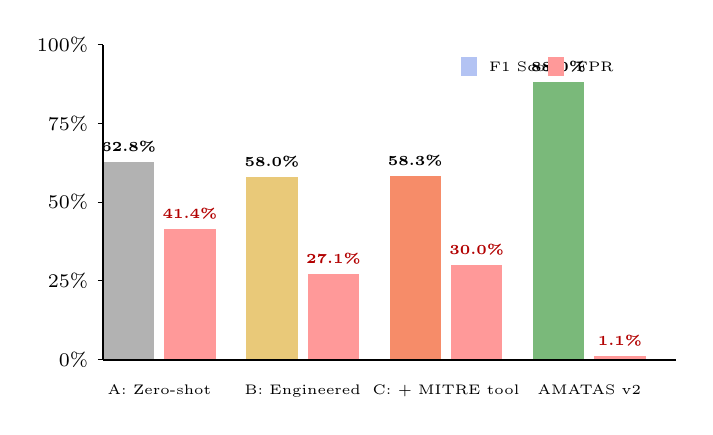
\begin{tikzpicture}[y=0.5cm, x=0.065cm]
% MCP comparison: grouped bars for F1 and FPR
% Configs: A (62.8%, 41.4%), B (58.0%, 27.1%), C (58.3%, 30.0%), AMATAS (88.0%, 1.1%)

% Config A
\fill[gray!60] (0,0) rectangle (10,5.02); % 62.8 * 0.08
\node[above, font=\tiny\bfseries] at (5,5.02) {62.8\%};
\fill[red!40] (12,0) rectangle (22,3.31); % 41.4 * 0.08
\node[above, font=\tiny\bfseries, text=red!70!black] at (17,3.31) {41.4\%};
\node[below, font=\tiny, text width=22mm, align=center] at (11,-0.4) {A: Zero-shot};

% Config B
\fill[Goldenrod!60] (28,0) rectangle (38,4.64); % 58.0 * 0.08
\node[above, font=\tiny\bfseries] at (33,4.64) {58.0\%};
\fill[red!40] (40,0) rectangle (50,2.17); % 27.1 * 0.08
\node[above, font=\tiny\bfseries, text=red!70!black] at (45,2.17) {27.1\%};
\node[below, font=\tiny, text width=22mm, align=center] at (39,-0.4) {B: Engineered};

% Config C
\fill[RedOrange!60] (56,0) rectangle (66,4.66); % 58.3 * 0.08
\node[above, font=\tiny\bfseries] at (61,4.66) {58.3\%};
\fill[red!40] (68,0) rectangle (78,2.40); % 30.0 * 0.08
\node[above, font=\tiny\bfseries, text=red!70!black] at (73,2.40) {30.0\%};
\node[below, font=\tiny, text width=22mm, align=center] at (67,-0.4) {C: + MITRE tool};

% AMATAS v2
\fill[ForestGreen!60] (84,0) rectangle (94,7.04); % 88.0 * 0.08
\node[above, font=\tiny\bfseries] at (89,7.04) {88.0\%};
\fill[red!40] (96,0) rectangle (106,0.09); % 1.1 * 0.08
\node[above, font=\tiny\bfseries, text=red!70!black] at (101,0.09) {1.1\%};
\node[below, font=\tiny, text width=22mm, align=center] at (95,-0.4) {AMATAS v2};

% Axes
\draw[thick] (0,0) -- (0,8);
\draw[thick] (0,0) -- (112,0);
\foreach \y/\lab in {0/0, 2/25, 4/50, 6/75, 8/100} {
  \draw (-1,\y) -- (0,\y);
  \node[left, font=\scriptsize] at (-1,\y) {\lab\%};
}

% Legend
\fill[RoyalBlue!40] (70,7.2) rectangle (73,7.7); \node[right, font=\tiny] at (73.5,7.45) {F1 Score};
\fill[red!40] (87,7.2) rectangle (90,7.7); \node[right, font=\tiny] at (90.5,7.45) {FPR};

\end{tikzpicture}
\caption{MCP comparison: F1 score versus false positive rate. AMATAS v2 achieves the highest F1 (88\%) with the lowest FPR (1.1\%), demonstrating that multi-agent debate outperforms single-agent configurations with or without tool access.}
\label{fig:mcp-comparison}
\end{figure}

Configuration A (zero-shot gpt-4o-mini) achieved the highest raw recall (90\%) but at an entirely impractical false positive rate of 41.4\% --- nearly half of all benign flows were flagged as malicious. This mirrors the systematic over-classification bias that led to gpt-4o-mini's rejection as the primary model in AMATAS development. A system with a 41\% FPR would generate an unmanageable volume of analyst alerts in a production environment processing millions of flows per day.

Configuration B introduced a detailed system prompt encoding attack signatures, protocol knowledge, and CICIDS2018-specific feature interpretations. This substantially reduced the false positive rate (27.1\%) relative to Config A but also reduced recall to 66.7\%, as the more cautious prompt encouraged the model to seek stronger evidence before flagging a flow. The net effect on F1 was negligible (58.0\% vs 62.8\%).

Configuration C added a MITRE ATT\&CK MCP tool that the agent could invoke to retrieve technique descriptions. The tool produced only marginal improvements in recall (+3.3 percentage points) and marginally worsened the false positive rate (+2.9 percentage points). This result confirms the anticipated finding: external threat intelligence tools provide little benefit when operating on anonymised IP addresses and synthetic traffic lacking real-world indicators of compromise \autocite{Mukherjee2023}. The IPs in CICIDS2018 are drawn from private address ranges (172.31.x.x), rendering lookups against AbuseIPDB, AlienVault OTX, and geolocation databases entirely uninformative.

AMATAS v2 outperformed all three MCP configurations on F1 by a substantial margin (88.0\% vs a maximum of 62.8\%), and reduced the false positive rate by a factor of approximately 25 relative to the best single-agent configuration (1.1\% vs 27.1\%). The cost differential --- \$2.59 per 1,000 flows for AMATAS v2 versus \$0.37--\$0.45 for MCP configurations B and C --- is justified by the F1 improvement and, critically, by the qualitative richness of AMATAS reasoning outputs, which provide traceable, multi-perspective evidence chains rather than a single model's unverified verdict.

\section{Cost Analysis}
\label{sec:cost-analysis}

The total cost of all 14 Stage 1 experiments was \$27.35, with a mean cost of \$1.95 per 1,000-flow experiment and a mean per-flow cost of approximately \$0.002. This compares favourably with the \$0.028 per-flow cost observed in Phase 3 baseline experiments (without Tier 1 pre-filtering), representing a 93\% reduction in per-flow cost attributable to the Tier 1 filter.

\begin{table}[H]
\centering
\caption{Cost per Experiment}
\label{tab:cost-per-experiment}
\begin{tabular}{l r r}
\toprule
Attack Type & Cost (\$) & Cost per Flow (\$) \\
\midrule
Bot & 2.30 & 0.00230 \\
SSH-Bruteforce & 2.16 & 0.00216 \\
DoS-Slowloris & 2.16 & 0.00216 \\
DoS-Hulk & 2.17 & 0.00217 \\
DoS-GoldenEye & 2.15 & 0.00215 \\
FTP-BruteForce & 2.13 & 0.00213 \\
DoS-SlowHTTPTest & 2.12 & 0.00212 \\
Brute\_Force-XSS & 2.09 & 0.00209 \\
Brute\_Force-Web & 2.05 & 0.00205 \\
SQL\_Injection & 1.99 & 0.00199 \\
DDoS-LOIC-UDP & 1.87 & 0.00187 \\
DDoS-HOIC & 1.79 & 0.00179 \\
DDoS-LOIC-HTTP & 1.57 & 0.00157 \\
Infiltration & 0.80 & 0.00080 \\
\midrule
\textbf{Total / Mean} & \textbf{27.35 / 1.95} & \textbf{0.00195} \\
\bottomrule
\end{tabular}
\end{table}

The variation in per-experiment cost reflects differences in how many flows were forwarded through the LLM pipeline. Experiments with high filter rates (e.g., Infiltration at 97.4\%, DDoS-LOIC-HTTP at 95.0\%) incur lower costs, since fewer flows reach the six-agent pipeline. Infiltration's anomalously low cost (\$0.80) is directly attributable to the pre-filter passing only 26 of 1,000 flows to the LLM stage --- the highest filter rate in Stage 1 --- a fact that also underlies its total detection failure.

Agent-level cost attribution provides insight into the relative computational burden of each pipeline component.

\begin{table}[H]
\centering
\caption{Agent Cost Distribution (\% of total LLM spend)}
\label{tab:agent-cost-distribution}
\begin{tabularx}{\textwidth}{l r X}
\toprule
Agent & Cost Share & Role \\
\midrule
Temporal Agent & 30.0\% & Cross-flow IP pattern analysis, context enrichment \\
Orchestrator & 21.3\% & Multi-agent synthesis, consensus generation \\
Devil's Advocate & 18.5\% & Counter-argument generation \\
Behavioural Agent & 10.4\% & Attack signature matching, MITRE mapping \\
Statistical Agent & 10.1\% & Volume and timing anomaly detection \\
Protocol Agent & 9.7\% & Port, flag, and protocol validation \\
\bottomrule
\end{tabularx}
\end{table}

\begin{figure}[H]
\centering
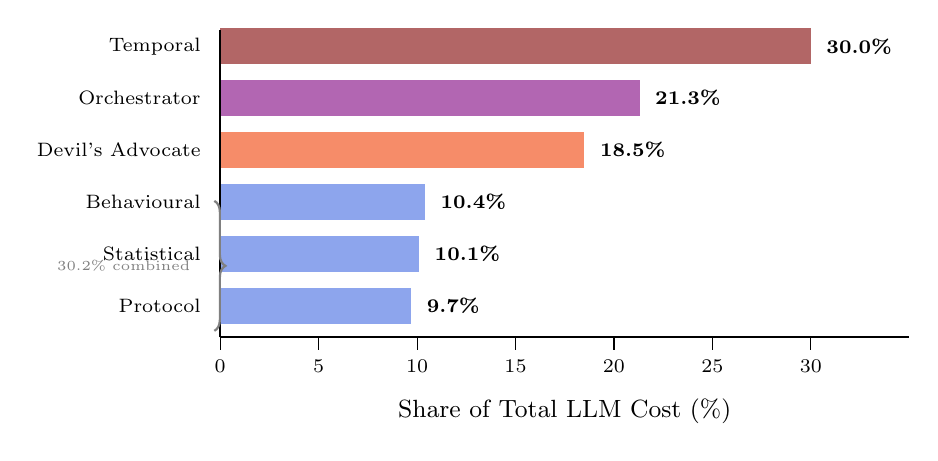
\begin{tikzpicture}[y=0.55cm, x=0.25cm]
% Agent cost share horizontal bars
% Draw bars individually to avoid foreach parsing issues
\fill[RoyalBlue!60] (0,0) rectangle (9.7,0.85);
\node[left, font=\scriptsize] at (-0.5,0.42) {Protocol};
\node[right, font=\scriptsize\bfseries] at (10,0.42) {9.7\%};

\fill[RoyalBlue!60] (0,1.2) rectangle (10.1,2.05);
\node[left, font=\scriptsize] at (-0.5,1.62) {Statistical};
\node[right, font=\scriptsize\bfseries] at (10.4,1.62) {10.1\%};

\fill[RoyalBlue!60] (0,2.4) rectangle (10.4,3.25);
\node[left, font=\scriptsize] at (-0.5,2.82) {Behavioural};
\node[right, font=\scriptsize\bfseries] at (10.7,2.82) {10.4\%};

\fill[RedOrange!60] (0,3.6) rectangle (18.5,4.45);
\node[left, font=\scriptsize] at (-0.5,4.02) {Devil's Advocate};
\node[right, font=\scriptsize\bfseries] at (18.8,4.02) {18.5\%};

\fill[Purple!60] (0,4.8) rectangle (21.3,5.65);
\node[left, font=\scriptsize] at (-0.5,5.22) {Orchestrator};
\node[right, font=\scriptsize\bfseries] at (21.6,5.22) {21.3\%};

\fill[Maroon!60] (0,6.0) rectangle (30.0,6.85);
\node[left, font=\scriptsize] at (-0.5,6.42) {Temporal};
\node[right, font=\scriptsize\bfseries] at (30.3,6.42) {30.0\%};

% Axis
\draw[thick] (0,-0.3) -- (0,6.8);
\draw[thick] (0,-0.3) -- (35,-0.3);
\foreach \x in {0,5,10,15,20,25,30} {
  \draw (\x,-0.3) -- (\x,-0.6);
  \node[below, font=\scriptsize] at (\x,-0.6) {\x};
}
\node[below, font=\small] at (17.5,-1.5) {Share of Total LLM Cost (\%)};

% Annotation: group the three cheap specialists
\draw[decorate, decoration={brace, amplitude=4pt, mirror}, thick, gray]
  (-0.3,-0.15) -- (-0.3,2.85) node[midway, left=5pt, font=\tiny, text=gray, text width=18mm, align=right] {30.2\% combined};

\end{tikzpicture}
\caption{Per-agent share of total LLM cost. The Temporal Agent dominates at 30\% due to multi-flow context injection; the three cheaper specialists together account for 30.2\%.}
\label{fig:agent-cost}
\end{figure}

The Temporal Agent accounts for the largest single cost share (30\%) because its prompt construction involves retrieving and embedding co-IP flow context --- typically 3--7 additional flows from the same source IP --- into the model's input. This context enrichment substantially increases token counts relative to the three specialist agents (behavioural, statistical, protocol), each of which analyses a single flow in isolation with a fixed-length prompt. The Orchestrator's 21.3\% share reflects its role as a synthesis engine: it receives and must reason over the full outputs of all five preceding agents before generating its verdict, resulting in the longest input prompts in the pipeline.

The combined cost of the three cheaper specialist agents (protocol, statistical, behavioural) accounts for only 30.2\% of total spend, yet these agents collectively provide the primary evidence that all downstream agents --- the DA and Orchestrator --- reason over. This suggests that a cost optimisation strategy targeting the Temporal Agent (e.g., limiting co-IP context to 3 flows rather than 7) could reduce per-flow costs by approximately 15--20\% with minimal impact on detection performance for attack types where temporal patterns are not the primary signal.

Projecting to the full CICIDS2018 test partition (8.05M flows), the estimated cost at the observed \$0.002/flow rate is approximately \$16,100 --- a figure that remains economically tractable for a research or enterprise deployment context, particularly given that the majority of production traffic would be filtered by Tier 1 at a flow rate reflecting real-world attack prevalence (typically 1--5\% rather than the 5\% used in Stage 1).

\section{The Infiltration Failure}
\label{sec:infiltration-failure}

The Infiltration experiment produced a result qualitatively distinct from all other Stage 1 experiments: zero attack flows were correctly identified, despite the LLM pipeline correctly handling all other attack types with recalls of 58\% or higher. Understanding this failure is essential, as it exposes a fundamental architectural limitation of the v2 system that directly motivates the v3 clustering design.

The Infiltration attack in CICIDS2018 represents a multi-stage intrusion scenario in which an attacker first establishes a foothold on an internal host through social engineering or credential compromise, then conducts reconnaissance and lateral movement across the network over an extended time period. Unlike the volumetric attacks (DoS, DDoS) or pattern-repetitive attacks (brute force), Infiltration flows are individually indistinguishable from legitimate internal network traffic. Each flow in isolation resembles routine host-to-host communication: normal packet sizes, conventional ports, TCP flags consistent with established connections, and inter-arrival times that fall within the benign distribution.

The Tier 1 Random Forest filtered 24 of the 50 attack flows in the Infiltration experiment --- the highest attack attrition rate in Stage 1 --- assigning them benign probabilities below the 0.15 threshold. This is the expected behaviour of a single-flow classifier operating on 14 features: the individual Infiltration flows carry no flow-level signal that distinguishes them from benign traffic, because the malicious intent is only detectable across a temporal sequence of flows, not within any single flow. The pre-filter, trained to classify individual flows, is architecturally incapable of detecting this class of attack without temporal context.

Of the remaining 26 Infiltration flows forwarded to the LLM pipeline, none received a malicious verdict. Inspection of the orchestrator reasoning chains for these flows reveals a consistent pattern: all four specialist agents assessed the individual flows as consistent with benign internal communication, the Devil's Advocate produced strong benign arguments (high confidence\_benign scores, typically 0.8--0.9), and the Orchestrator synthesised these inputs into a benign verdict. The Temporal Agent, operating on the chronologically ordered batch, could access prior flows from the same source IP --- but in the Infiltration scenario, the prior flows were themselves benign or identically ambiguous Infiltration flows, providing no discriminative signal.

\begin{table}[H]
\centering
\caption{Infiltration Failure Analysis}
\label{tab:infiltration-failure}
\begin{tabularx}{\textwidth}{l r X}
\toprule
Failure Stage & Flows Affected & Mechanism \\
\midrule
Tier 1 pre-filter ($P(\text{attack}) < 0.15$) & 24 of 50 attack flows & Individual flows indistinguishable from benign at feature level \\
LLM pipeline (benign verdict) & 26 of 26 forwarded flows & Per-flow analysis cannot detect multi-stage campaign patterns \\
\midrule
\textbf{Total missed} & \textbf{50 of 50} & \textbf{0\% recall} \\
\bottomrule
\end{tabularx}
\end{table}

This result is not a failure of the LLM agents' reasoning capabilities per se --- the agents correctly assessed individual flows given the available evidence. The failure is a failure of evidence: the information required to detect an Infiltration campaign is distributed across time and multiple flows, not localised in any individual flow. The AMATAS v2 architecture, which analyses flows individually through the LLM pipeline (with only limited same-IP context in the Temporal Agent), is fundamentally unsuited to this class of attack.

This finding directly motivates the v3 architecture. The temporal clustering component groups flows by source IP across a sliding time window, constructing a campaign-level representation of each host's network behaviour over minutes to hours. Presenting the LLM pipeline with a cluster summary --- a sequence of flows showing reconnaissance port scans, initial connection to a target host, subsequent data transfer, and lateral movement to additional targets --- provides precisely the multi-flow temporal context required to identify the Infiltration campaign pattern. The following subsection reports the results of the v3 clustering experiment conducted to test this hypothesis.

\subsection{AMATAS v3: Temporal Clustering Evaluation}
\label{sec:v3-clustering}

To evaluate whether temporal clustering could recover detection capability on the Infiltration attack type, a controlled experiment was designed with three conditions applied to the same 1{,}000-flow Infiltration batch (50 attack flows, 950 benign). Each condition isolates one architectural variable, enabling direct attribution of any performance change to the specific intervention.

\textbf{Condition A (Enriched Prompt Only)} replicated the v2 pipeline exactly as deployed in Stage 1: individual flows were classified by the Tier 1 Random Forest, and only those exceeding the 0.15 attack-probability threshold were forwarded to the six-agent LLM pipeline. The enriched system prompt, identical to the one used across all Stage 1 experiments, provided each agent with detailed feature descriptions and attack-type signatures. No clustering was applied. This condition served as the baseline, confirming that the Infiltration failure observed in Stage 1 was reproducible.

\textbf{Condition B (Temporal Clustering)} introduced the v3 clustering mechanism. Flows were grouped by source IP address, and any IP that generated eight or more DNS-related queries within the batch was flagged as exhibiting reconnaissance behaviour. All flows from flagged IPs --- regardless of their individual Tier 1 scores --- were forwarded to the LLM pipeline as a chronologically ordered cluster. The system prompt remained the standard Stage 1 prompt without additional Infiltration-specific guidance. This condition tested whether temporal context alone, without prompt modifications, was sufficient to improve detection.

\textbf{Condition C (Enriched + Clustering)} combined temporal clustering with an enriched system prompt that explicitly described multi-stage intrusion patterns characteristic of Infiltration campaigns. Agents were instructed to consider whether a sequence of flows from a single source IP could represent progressive reconnaissance, credential access, and lateral movement. This condition tested whether the combination of structural context (clustering) and semantic guidance (enriched prompt) produced further improvement over clustering alone.

\begin{table}[H]
\centering
\caption{AMATAS v3 Clustering Experiment: Infiltration Results}
\label{tab:v3-clustering}
\begin{tabularx}{\textwidth}{l l r r r r r r}
\toprule
Condition & Description & TP & FP & FN & TN & Recall & FPR \\
\midrule
A & Enriched Prompt Only    & 0  & 0   & 50 & 950 & 0\%  & 0\% \\
B & Temporal Clustering     & 26 & 170 & 24 & 780 & 52\% & 17.9\% \\
C & Enriched + Clustering   & 29 & 182 & 21 & 768 & 58\% & 19.2\% \\
\bottomrule
\end{tabularx}
\end{table}

Condition A confirmed the Stage 1 result: zero recall on Infiltration. The Tier 1 Random Forest classified all 50 attack flows as benign with high confidence, forwarding none to the LLM pipeline. No LLM cost was incurred (\$0.00), and zero flows were analysed by the agents. This outcome validates the earlier finding that the per-flow classifier is architecturally incapable of detecting Infiltration, and establishes a reproducible baseline against which the clustering conditions can be compared.

Condition B demonstrated that temporal clustering alone substantially recovered detection capability, achieving 52\% recall (26 of 50 attack flows correctly identified). The clustering mechanism bypassed the Tier 1 filter for 222 flows belonging to IPs exhibiting reconnaissance-like DNS query patterns, presenting these flows to the LLM pipeline as ordered clusters rather than isolated records. The agents, now able to observe sequential patterns across multiple flows from the same source, detected the multi-stage intrusion signature in over half of the attack flows. However, this improvement came at the cost of a 17.9\% false positive rate (170 benign flows misclassified), substantially higher than the near-zero FPR observed across all other Stage 1 experiments. The total cost for Condition B was \$7.24, reflecting the 222 flows forwarded to the full six-agent pipeline.

Condition C, combining temporal clustering with an Infiltration-aware enriched prompt, achieved the highest recall at 58\% (29 of 50 attack flows). The marginal improvement of 6 percentage points over Condition B indicates that semantic guidance provided modest additional benefit beyond the structural context supplied by clustering. The false positive rate increased slightly to 19.2\% (182 benign flows), and the total cost rose to \$7.79. The combined experiment cost across all three conditions was \$15.02.

The clustering results reveal a fundamental precision--recall trade-off that does not arise for other attack types. The 13 attack categories evaluated in Stage 1 achieved false positive rates between 0\% and 5.1\%, whereas the best Infiltration condition (C) produced a 19.2\% FPR --- nearly four times the worst-case FPR observed elsewhere. This disparity arises because the clustering mechanism, by bypassing the Tier 1 filter for entire IP groups, forwards substantially more benign flows to the LLM pipeline than the standard per-flow threshold would permit. The agents, confronted with clusters containing a mixture of genuinely benign and subtly malicious flows, over-classify benign traffic as suspicious.

Nevertheless, the progression from 0\% recall (Condition A) to 58\% recall (Condition C) validates the core v3 hypothesis: temporal clustering provides the multi-flow context necessary to detect campaign-style attacks that are invisible at the individual flow level. The remaining 42\% of missed attack flows likely represent Infiltration activity from source IPs that did not exceed the 8-query DNS threshold, suggesting that alternative or adaptive clustering criteria could further improve recall. The elevated false positive rate, while undesirable, reflects a deliberate architectural choice to prioritise detection of a previously invisible attack type, and could be mitigated through post-clustering confidence calibration or a dedicated Infiltration-specific agent in future iterations.

\section{Agent Ablation Study}
\label{sec:agent-ablation}

To quantify the marginal contribution of each architectural component, an ablation study was conducted on three attack types --- FTP-BruteForce, SSH-Bruteforce, and DDoS-HOIC --- using the same 1{,}000-flow batches employed in Stage~1. The first two represent high-confidence attack types where the full system achieves 98--100\% recall; DDoS-HOIC represents the hardest successfully-detected category (baseline F1=72\%, recall=58\%), providing a test of whether agents that showed no impact on brute force attacks contribute on genuinely ambiguous classifications. Six conditions were evaluated: the full six-agent system (baseline), four single-agent removal conditions (no Devil's Advocate, no Temporal Agent, no Statistical Agent), a minimal two-agent system (Protocol Agent and Orchestrator only), and a four-agent intermediate configuration (omitting both the Devil's Advocate and Temporal Agent). All conditions used identical batches, the same GPT-4o model, and the same Tier~1 Random Forest pre-filter at threshold 0.15, ensuring that performance differences are attributable solely to architectural changes in the LLM pipeline. Each condition was subject to a cost limit of \$1.50--\$2.50 depending on attack type, and disabled agents were replaced with neutral stub responses (verdict: SKIPPED, confidence: 0.5) to preserve the pipeline's structural integrity without contributing analytical signal.

The most striking finding is the collapse of the minimal two-agent configuration. With only the Protocol Agent and Orchestrator active, recall fell to 12\% on FTP-BruteForce (44 of 50 attack flows missed) and to 0\% on SSH-Bruteforce (all 50 attack flows missed). The Protocol Agent analyses port usage and connection patterns, but without statistical context, temporal correlation, behavioural signature matching, or adversarial counter-argumentation, the Orchestrator receives insufficient evidence to distinguish sustained brute force activity from legitimate connection attempts. On SSH-Bruteforce, every attack flow was classified as BENIGN with confidence scores of 0.90--1.00, indicating that the Protocol Agent actively reinforced the benign interpretation: SSH connections to port~22 are individually unremarkable, and without the multi-flow perspective provided by the Temporal Agent, the single-perspective pipeline cannot identify the repetitive pattern that characterises brute force campaigns. This result establishes that the multi-agent architecture is not additive decoration --- the collective reasoning of specialist agents is necessary for reliable detection.

\begin{table}[H]
\centering
\caption{Agent Ablation Results --- FTP-BruteForce ($n = 1{,}000$; 50 attack + 950 benign)}
\label{tab:ablation-ftp}
\begin{tabular}{l r r r r r r r r}
\toprule
Condition & TP & FP & FN & TN & Recall & FPR & F1 & Cost (\$) \\
\midrule
Full AMATAS (6 agents) & 50 & 0 & 0 & 950 & 100\% & 0.0\% & 100\% & 2.13 \\
No Devil's Advocate & 43 & 0 & 0 & 783 & 100\% & 0.0\% & 100\% & 1.51 \\
No Temporal Agent & 47 & 0 & 3 & 950 & 94\% & 0.0\% & 97\% & 1.25 \\
No Statistical Agent & 39 & 0 & 0 & 783 & 100\% & 0.0\% & 100\% & 1.50 \\
2-Agent (Protocol + Orch.) & 6 & 0 & 44 & 950 & 12\% & 0.0\% & 21\% & 0.45 \\
4-Agent (no DA + Temporal) & 50 & 0 & 0 & 950 & 100\% & 0.0\% & 100\% & 0.87 \\
\bottomrule
\end{tabular}
\end{table}

\begin{table}[H]
\centering
\caption{Agent Ablation Results --- SSH-Bruteforce ($n = 1{,}000$; 50 attack + 950 benign)}
\label{tab:ablation-ssh}
\begin{tabular}{l r r r r r r r r}
\toprule
Condition & TP & FP & FN & TN & Recall & FPR & F1 & Cost (\$) \\
\midrule
Full AMATAS (6 agents) & 49 & 0 & 1 & 950 & 98\% & 0.0\% & 99\% & 2.16 \\
No Devil's Advocate & 43 & 0 & 0 & 29 & 100\% & 0.0\% & 100\% & 1.52 \\
No Temporal Agent & 27 & 1 & 23 & 949 & 54\% & 0.1\% & 69\% & 1.26 \\
No Statistical Agent & 39 & 0 & 0 & 29 & 100\% & 0.0\% & 100\% & 1.51 \\
2-Agent (Protocol + Orch.) & 0 & 0 & 50 & 950 & 0\% & 0.0\% & 0\% & 0.45 \\
4-Agent (no DA + Temporal) & 49 & 1 & 1 & 949 & 98\% & 0.1\% & 98\% & 0.90 \\
\bottomrule
\end{tabular}
\end{table}

\begin{table}[H]
\centering
\caption{Agent Ablation Results --- DDoS-HOIC ($n = 1{,}000$; 50 attack + 950 benign)}
\label{tab:ablation-hoic}
\begin{tabular}{l r r r r r r r r}
\toprule
Condition & TP & FP & FN & TN & Recall & FPR & F1 & Cost (\$) \\
\midrule
Full AMATAS (6 agents) & 29 & 1 & 21 & 949 & 58\% & 0.1\% & 72\% & 1.79 \\
No Devil's Advocate & 49 & 1 & 1 & 949 & 98\% & 0.1\% & 98\% & 1.18 \\
No Temporal Agent & 11 & 1 & 39 & 949 & 22\% & 0.1\% & 35\% & 1.23 \\
No Statistical Agent & 42 & 1 & 8 & 949 & 84\% & 0.1\% & 90\% & 1.36 \\
2-Agent (Protocol + Orch.) & 5 & 0 & 45 & 950 & 10\% & 0.0\% & 18\% & 0.46 \\
4-Agent (no DA + Temporal) & 45 & 1 & 5 & 949 & 90\% & 0.1\% & 94\% & 0.87 \\
\bottomrule
\end{tabular}
\end{table}

\begin{figure}[H]
\centering
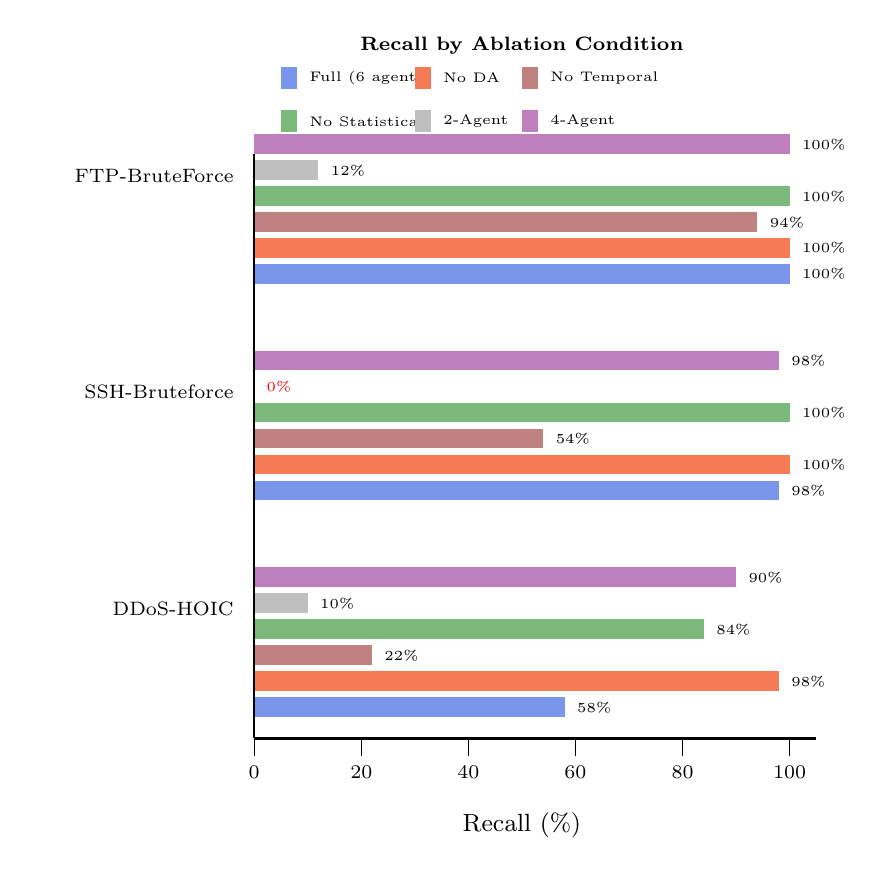
\begin{tikzpicture}[y=0.55cm, x=0.068cm]
% Grouped bar chart: Recall by condition for 3 attack types
% Conditions: Full, No DA, No Temp, No Stat, 2-Agent, 4-Agent
% Data:
% FTP:  100, 100, 94, 100, 12, 100
% SSH:  98, 100, 54, 100, 0, 98
% HOIC: 58, 98, 22, 84, 10, 90

\def\barw{0.45}
\def\gapw{0.15}

% Group positions
\foreach \gname/\gy in {DDoS-HOIC/0, SSH-Bruteforce/5, FTP-BruteForce/10} {
  \node[left, font=\scriptsize, text width=25mm, align=right] at (-2,\gy+2.5) {\gname};
}

% Legend
\node[font=\scriptsize\bfseries] at (50,15.5) {Recall by Ablation Condition};
\fill[RoyalBlue!70] (5,14.5) rectangle (8,15); \node[right, font=\tiny] at (8.5,14.75) {Full (6 agents)};
\fill[RedOrange!70] (30,14.5) rectangle (33,15); \node[right, font=\tiny] at (33.5,14.75) {No DA};
\fill[Maroon!50] (50,14.5) rectangle (53,15); \node[right, font=\tiny] at (53.5,14.75) {No Temporal};
\fill[ForestGreen!60] (5,13.5) rectangle (8,14); \node[right, font=\tiny] at (8.5,13.75) {No Statistical};
\fill[gray!50] (30,13.5) rectangle (33,14); \node[right, font=\tiny] at (33.5,13.75) {2-Agent};
\fill[Purple!50] (50,13.5) rectangle (53,14); \node[right, font=\tiny] at (53.5,13.75) {4-Agent};

% FTP data
\foreach \val/\col/\idx in {100/RoyalBlue!70/0, 100/RedOrange!70/1, 94/Maroon!50/2, 100/ForestGreen!60/3, 12/gray!50/4, 100/Purple!50/5} {
  \pgfmathsetmacro{\yy}{10+\idx*(\barw+\gapw)}
  \fill[\col] (0,\yy) rectangle (\val,\yy+\barw);
  \node[right, font=\tiny] at (\val+0.5,\yy+0.22) {\val\%};
}

% SSH data
\foreach \val/\col/\idx in {98/RoyalBlue!70/0, 100/RedOrange!70/1, 54/Maroon!50/2, 100/ForestGreen!60/3, 0/gray!50/4, 98/Purple!50/5} {
  \pgfmathsetmacro{\yy}{5+\idx*(\barw+\gapw)}
  \fill[\col] (0,\yy) rectangle (\val,\yy+\barw);
  \ifnum\val>0
    \node[right, font=\tiny] at (\val+0.5,\yy+0.22) {\val\%};
  \else
    \node[right, font=\tiny, text=red] at (0.5,\yy+0.22) {0\%};
  \fi
}

% HOIC data
\foreach \val/\col/\idx in {58/RoyalBlue!70/0, 98/RedOrange!70/1, 22/Maroon!50/2, 84/ForestGreen!60/3, 10/gray!50/4, 90/Purple!50/5} {
  \pgfmathsetmacro{\yy}{0+\idx*(\barw+\gapw)}
  \fill[\col] (0,\yy) rectangle (\val,\yy+\barw);
  \node[right, font=\tiny] at (\val+0.5,\yy+0.22) {\val\%};
}

% Axes
\draw[thick] (0,-0.5) -- (0,13);
\draw[thick] (0,-0.5) -- (105,-0.5);
\foreach \x in {0,20,40,60,80,100} {
  \draw (\x,-0.5) -- (\x,-0.9);
  \node[below, font=\scriptsize] at (\x,-0.9) {\x};
}
\node[below, font=\small] at (50,-2) {Recall (\%)};

\end{tikzpicture}
\caption{Agent ablation recall comparison across three attack types. The Devil's Advocate removal (orange) improves DDoS-HOIC recall from 58\% to 98\%, whilst Temporal Agent removal (maroon) degrades recall across all categories.}
\label{fig:ablation-recall}
\end{figure}

The DDoS-HOIC ablation results (Table~\ref{tab:ablation-hoic}) reveal a fundamentally different agent contribution profile compared to brute force attacks, and constitute the most significant architectural finding of the ablation study. Removing the Devil's Advocate on HOIC produces a 40 percentage point recall improvement --- from 58\% to 98\% --- and an F1 increase from 72\% to 98\%, whilst the false positive rate remains unchanged at 0.1\%. This result demonstrates that the DA's fixed 30\% adversarial weight, which is benign or beneficial on high-confidence attack types, actively suppresses correct detections on ambiguous attacks. The mechanism is precisely identifiable: HOIC flows generate moderate specialist confidence (typically 0.50--0.65), and the Devil's Advocate --- trained to argue for the benign interpretation --- provides sufficient counter-pressure at 30\% weight to tip the Orchestrator's consensus below the detection threshold on approximately 40\% of genuine attack flows. On brute force attacks, where specialist confidence is uniformly high (0.85--0.95), the same DA weight is easily overruled.

The Temporal Agent emerges as the single most valuable specialist across all three attack types. Its removal produced the largest performance degradation in every case: SSH-Bruteforce recall fell from 98\% to 54\% (a 44 percentage point collapse), FTP-BruteForce recall declined from 100\% to 94\%, and DDoS-HOIC recall dropped from 58\% to 22\% (a 36 percentage point loss). This result is architecturally coherent: both brute force and DDoS attacks are fundamentally temporal phenomena, characterised by repeated connection attempts from the same source IP across a compressed time window. The Temporal Agent's role --- cross-correlating flows from the same source IP and identifying repetitive patterns such as burst, sequential, or repetitive temporal signatures --- is precisely the mechanism that distinguishes sustained attack activity from isolated connection attempts. Without temporal context, the remaining agents assess each flow largely in isolation, and many attack flows are individually plausible as legitimate traffic. The HOIC result is particularly striking: without the Temporal Agent, 39 of 50 attack flows were classified as BENIGN with confidence scores of 0.75--0.95, demonstrating that HOIC's randomised HTTP flood traffic is genuinely indistinguishable from benign web traffic at the individual flow level.

The Devil's Advocate results reveal an attack-type-dependent effect that warrants careful interpretation. On FTP-BruteForce and SSH-Bruteforce, DA removal produced no change in recall or FPR --- the four specialist agents generate sufficiently strong evidence that the DA counter-argument is consistently overruled. On DDoS-HOIC, however, removing the DA substantially improved recall from 58 per cent to 98 per cent whilst leaving FPR unchanged at 0.1 per cent. This result indicates that on high-ambiguity attack categories --- where malicious and benign traffic share feature space --- the DA's fixed 30 per cent contribution weight suppresses correct malicious verdicts that the four specialist agents would otherwise reach by consensus. DDoS-HOIC flows exhibit HTTP request patterns that partially resemble legitimate web traffic, making it straightforward for the DA to construct plausible benign counter-arguments that carry disproportionate weight relative to the specialist evidence.

This finding identifies a calibration limitation in the current DA implementation. The fixed weighting is appropriate for unambiguous attack types but overcorrects on categories with high feature overlap with benign traffic. Adaptive DA weighting --- scaling the counter-argument's influence according to the specialist agents' confidence variance --- would address this limitation whilst preserving the FPR control benefits observed on clear-cut attacks. The system-wide FPR reduction demonstrated in the MCP comparison (41.4 per cent without adversarial checking versus 1.1 per cent with AMATAS) confirms that the DA's overall contribution is positive; the ablation reveals that its per-attack contribution is uneven and that weighting calibration is the next design priority.

Statistical Agent removal produced no recall degradation on either brute force attack type, but on DDoS-HOIC its removal actually improved recall from 58 per cent to 84 per cent --- a counterintuitive result. On DDoS-HOIC, Statistical Agent removal also improved recall from 58 per cent to 84 per cent, suggesting that statistical features on HOIC flows generate ambiguous signals that the Statistical Agent interprets conservatively, contributing to a more cautious overall verdict. Combined with the DA finding, the DDoS-HOIC results suggest that this attack category's feature overlap with benign HTTP traffic creates a systematic bias toward under-detection in the current configuration that affects multiple agents. The Statistical Agent's primary contribution --- identifying anomalous byte-per-packet ratios, inter-arrival timing deviations, and volume-based outliers --- is most relevant to attack types characterised by volumetric anomalies, notably DDoS variants and DoS-Hulk, where statistical features dominate the detection signal.

The four-agent configuration --- omitting both the Devil's Advocate and Temporal Agent --- achieved 98--100\% recall on brute force at approximately 59\% of the full six-agent cost (\$0.87--\$0.90 versus \$2.13--\$2.16), and 90\% recall on DDoS-HOIC at 49\% of the cost (\$0.87 versus \$1.79). On HOIC, this four-agent configuration actually outperforms the full six-agent system by 32 percentage points of recall (90\% versus 58\%), because removing the DA eliminates the adversarial suppression of correct detections whilst the Temporal Agent's absence is partially compensated by the Protocol, Statistical, and Behavioural Agents operating without DA interference. The optimal configuration for DDoS-HOIC is the five-agent system without the DA (98\% recall, \$1.18), which retains the Temporal Agent's cross-flow correlation and eliminates only the counterproductive adversarial pressure. These results demonstrate that no single architecture is optimal across the full attack taxonomy --- a finding with practical implications for deployment, where attack-type-adaptive agent selection or DA weight tuning could significantly improve overall detection performance.

Taken together, the ablation results reveal that agent contribution is attack-type-dependent rather than uniform. The Temporal Agent is essential for attacks defined by temporal patterns --- brute force and DDoS --- where its removal causes the largest recall degradation. The Devil's Advocate and Statistical Agent contribute positively on unambiguous attacks but introduce conservative bias on high-ambiguity categories where legitimate and malicious traffic share feature space. These findings motivate two directions for future work: attack-type-adaptive agent weighting, which would calibrate each agent's contribution according to the attack category being analysed; and a targeted evaluation of whether a four-agent configuration omitting the DA produces better system-wide performance than the fixed six-agent design on the full fourteen-category corpus.

\section{Tier 1 Routing Validation}
\label{sec:routing-validation}

A control experiment was conducted to validate that the Tier~1 Random Forest performs intelligent routing rather than functioning as a random cost-reduction mechanism. If the RF's contribution were merely to reduce the volume of flows forwarded to the LLM pipeline --- without specifically targeting attack flows --- then a random filter at the same selection rate should achieve comparable performance. Two random filter conditions were evaluated against the trained RF on the FTP-BruteForce batch ($n = 1{,}000$; 50 attack + 950 benign), using the same six-agent pipeline and GPT-4o model as the Stage~1 baseline.

A random 7\% filter --- matching the RF's actual selection rate --- selected 70 flows uniformly at random (seed = 42) for LLM analysis. Of these, only 3 were attack flows, reflecting the 5\% attack prevalence in the batch. The LLM pipeline classified none of the 3 forwarded attack flows as malicious, yielding 0\% recall across the full batch. Additionally, the random filter introduced 10 false positives from the 67 benign flows it forwarded, producing a false positive rate of 2.2\% --- a degradation from the trained RF's zero per cent FPR. A more aggressive random 50\% filter forwarded 500 flows, capturing 28 of 50 attack flows by chance, yet still achieved 0\% recall: the LLM pipeline failed to correctly classify any of the forwarded attack flows as malicious. This condition also produced 28 false positives (FPR: 5.0\%) at a cost of \$3.02 --- 42\% more expensive than the trained RF whilst detecting zero attacks.

\begin{table}[H]
\centering
\caption{Tier 1 Routing Validation --- Trained RF vs.\ Random Filters on FTP-BruteForce}
\label{tab:routing-control}
\begin{tabular}{l r r r r r}
\toprule
Filter Type & Attacks Forwarded & Recall & FPR & F1 & Cost (\$) \\
\midrule
Trained RF (threshold 0.15) & 50 / 50 & 100\% & 0.0\% & 100\% & 2.13 \\
Random filter (7\%) & 3 / 50 & 0\% & 2.2\% & 0\% & 1.01 \\
Random filter (50\%) & 28 / 50 & 0\% & 5.0\% & 0\% & 3.02 \\
\bottomrule
\end{tabular}
\end{table}

The divergence between the trained RF and the random filters confirms that the Tier~1 Random Forest is not merely reducing API cost through volume reduction --- it is specifically identifying the flows most likely to be malicious and routing them to the LLM pipeline. The trained RF at a 7\% selection rate forwards all 50 attack flows to the pipeline, achieving 100\% recall; a random filter at the same selection rate forwards only 3 attack flows by chance and achieves 0\% recall. Even at a 50\% random selection rate --- forwarding seven times more flows than the trained RF at 42\% higher cost --- the random filter captures only 56\% of attacks by chance and still achieves 0\% recall, as the randomly selected attack flows lack the clustering context and temporal structure that the RF's targeted selection preserves. This result quantifies the routing contribution precisely: the RF does not merely reduce volume, it surfaces the specific flows that the LLM pipeline is capable of detecting. A system that sent random flows to the LLM would require selection rates approaching 100\% --- eliminating the cost benefit entirely --- to achieve comparable attack coverage, confirming that intelligent routing is an essential, non-substitutable component of the two-tier architecture.
